\documentclass[a4paper]{article}
\usepackage[utf8]{inputenc}
\usepackage[russian]{babel}
\usepackage[T2]{fontenc}
\usepackage[warn]{mathtext}
\usepackage{graphicx}
\usepackage{amsmath}
\usepackage{floatflt}
\usepackage[left=20mm, top=20mm, right=20mm, bottom=20mm, footskip=10mm]{geometry}


\graphicspath{ {images/} }
\usepackage{multicol}
\setlength{\columnsep}{2cm}


\begin{document}

\begin{titlepage}
	\centering
	\vspace{5cm}
	{\scshape\LARGE Московский физико-технический институт \par}
	\vspace{4cm}
	{\scshape\Large Лабораторная работа \par}
	\vspace{1cm}
	{\huge\bfseries Исследование гальванометра \par}
	\vspace{1cm}
	\vfill
\begin{flushright}
	{\large выполнила студентка 653 группы ФФКЭ}\par
	\vspace{0.3cm}
	{\LARGE Карпова Татьяна}
\end{flushright}
	

	\vfill

% Bottom of the page
	Долгопрудный, 2017 г.
\end{titlepage}

\section{Цель работы}
Изучение работы высокочувствительного зеркального гальванометра магнитоэлектрической системы в режимах измерения постоянного тока и электрического заряда.

\section{В работе используются:}
\begin{itemize}
    \item зеркальный гальванометр с осветителем и шкалой
    \item источник постоянного напряжения
    \item делитель напряжения
    \item магазин сопротивлений
    \item эталонный конденсатор
    \item вольтметр
    \item переключатель
    \item ключи
    \item линейка
\end{itemize}

\section{Теоретические положения}

\textit{Баллистический гальванометр} -- электроизмерительный прибор магнитоэлектрической системы, отличающийся высокой чувствительностью к току и сравнительно большим периодом свободных колебаний. \par
На помещённую в магнитное поле обтекаемую током рамку гальванометра действуют момент закрученной нити, момент магнитных сил и тормозящий момент (зависит от сил сопротивления воздуха и от вихревых токов). Учитывая все эти моменты, уравнение движения рамки принимает вид
\begin{center}
    $\ddot \varphi + 2 \gamma \dot \varphi + \omega_0^2\varphi = KI $,
\end{center}
где $\gamma$ -- коэффициент затухания подвижной системы гальванометра, $\omega_0$ -- собственная частота колебаний рамки

Динамическая постоянная гальванометра определяется при пропускании через рамку постоянного тока:
\begin{center}
    $C_I = \frac{I}{\varphi} = \frac{D}{BSN}$,
\end{center}
где $B$ - индукция магнитного поля в рамке, $S$ - площадь одного витка рамки, $D$ - модуль кручения нити. \par
При пропускании коротких импульсов тока через баллистический гальванометр начальная скорость движения рамки пропорциональна электрическому заряду, прошедшему через рамку за всё время импульса. Отношение баллистических постоянных в критическом и свободном режимах равно $e$.

\section{Экспериментальная установка}
\subsection{Определение динамической постоянной}
\begin{figure}[h]
    \centering
    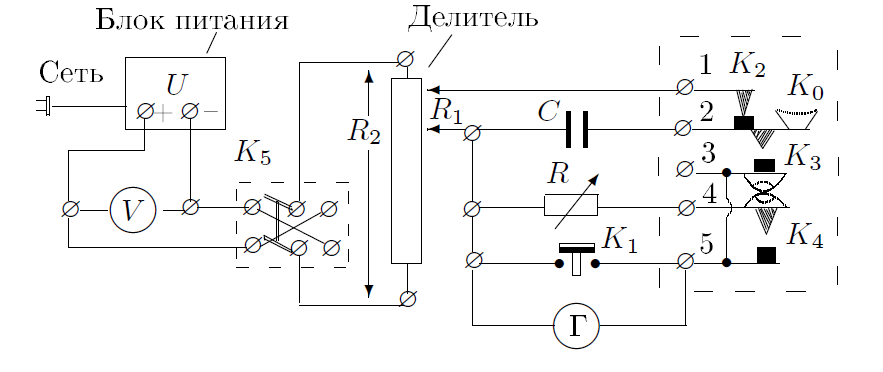
\includegraphics[width=10cm]{fig1.PNG}
    \caption{Схема установки для работы гальванометра в стационарном режиме}
    \label{fig:vac}
\end{figure}
Постоянное напряжение $U = 1,5$В снимается с блока питания и измеряется вольтметром $V$. Ключ $K_3$ позволяет менять величину тока через гальванометр Г, делитель напряжения - менять величину тока в широких пределах. Ключ $K_2$ служит для включения гальванометра, кнопка $K_1$ -- для его успокоения. Магазин сопротивлений $R$ позволяет менять режим работы гальванометра от колебательного до апериодического. \par
При малых $R_1$ сила тока, протекающего через гальванометр, может быть вычислена по формуле 
\begin{equation}
    I = U_0 \frac{R_1}{R_2} \frac{1}{R + R_0}.
\end{equation}
Динамическую постоянную вычисли по формуле 
\begin{equation}
    C_I = \frac{2aI}{x},
\end{equation}
где $a$ - расстояние от шкалы до зеркальца.

\subsection{Определение критического сопротивления гальванометра}
Выполняется с помощью той же цепи, что и на рис. 1. При больших $R$ движение рамки имеет колебательный характер, с уменьшением $R$ затухание увеличивается, и колебательный режим переходит в апериодический. \par
Найдём логарифмический декремент затухания колебаний рамки  $\Theta$.
\begin{equation}
    \Theta = ln\frac{x_n}{x_{n+1}} = \gamma T = \frac{2\pi \gamma}{\sqrt{\omega_0^2 - \gamma^2}} = \frac{2\pi R_3}{\sqrt{(R_0 + R)^2 - R_3^2}}
\end{equation}

Рассчитаем критическое сопротивление по графику в координатах $X = (R_0^2 + R)$, $Y = 1/\Theta^2$
\begin{equation}
    R_c_r = \frac{1}{2\pi}\sqrt{\frac{\triangle X}{\triangle Y}} - R_0
\end{equation}

\subsection{Определение баллистической постоянной и критического сопротивления гальванометра, работающего в баллистическом режиме}

Для изучения работы гальванометра в режиме измерения заряда используется схема, представленная на рис. 2.

\begin{figure}[h]
    \centering
    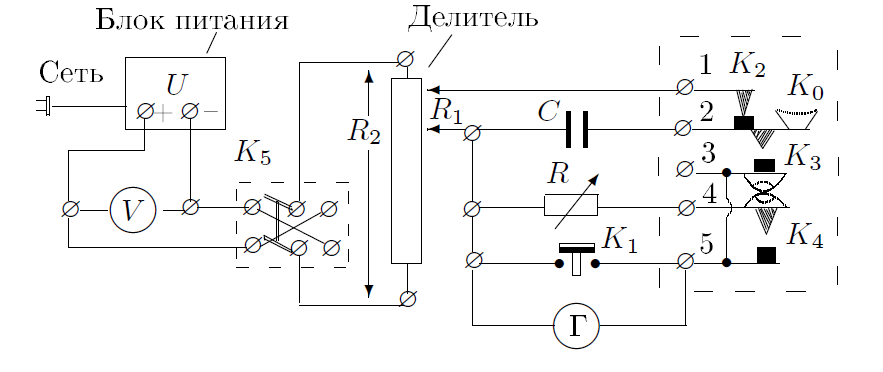
\includegraphics[width=10cm]{fig1.PNG}
    \caption{Схема установки для определения баллистической постоянной}
    \label{fig:vac}
\end{figure}

При нормальном положении кнопки $K_0$ конденсатор $C$ заряжается до напряжения
\begin{center}
    $U_c = \frac{R_1}{R_2}U_0$
\end{center}
Заряд конденсатора равен
\begin{center}
    $q = \frac{R_1}{R_2}U_0 C$
\end{center}
При нажатии на ключ $K_0$ конденсатор отключается от источника постоянного напряжения и подключается к гальванометру. К моменту замыкания ключа $K_4$ весь заряд успевает пройти через гальванометр, рамка получает начальную скорость. Баллистическая постоянная гальванометра определяется при критическом сопротивлении
\begin{equation}
    C_Q_c_r = \frac{q}{\varphi_{max cr}} = 2a\frac{R_1}{R_2} \frac{U_0 C}{l_{max cr}}
\end{equation}

\section{Ход работы}
\begin{enumerate}
    \item Подготовим к работе приборы, настроим гальванометр. Соберём схему согласно рис. 1. Снимем зависимость отклонения зайчика $x$ от сопротивления магазина $R$, увеличивая сопротивление магазина, но не меняя делителя. Результаты запишем в табл. 1. Ток в цепи рассчитаем по формуле (1) ($R_1/R_2 = 1/2000$, $U_0 = 1.47$ В, $R_0 = 280$ Ом.)
    
    \begin{table}[h]
    \centering
    \begin{center}
    \caption{Зависимость отклонения зайчика от сопротивления, постоянный ток}
    \end{center}
    \vspace{0.1cm}
    \label{tab:my_label}
    \begin{tabular}{ |p{1.4cm}||p{0.8cm}|p{0.8cm}|p{0.8cm}|p{0.8cm}|p{0.8cm}|p{0.8cm}|p{0.8cm}|p{0.8cm}|p{0.75cm}|p{0.75cm}|p{0.75cm}|p{0.75cm}|p{0.75cm}| }
 \hline
    $x$, мм & 161 & 144 & 133 & 119 & 109 & 99 & 78 & 63 & 52 & 25 & 15 & 12 & 2 \\
\hline
    $R$, кОм & 2.4 & 2.9 & 3.3 & 3.9 & 4.4 & 5 & 6.8 & 8.8 & 10.8 & 20.8 & 29.8 & 34 & 44 \\
\hline
    $I$, нА & 264.93 & 223.27 & 198.32 & 169.86 & 151.71 & 134.47 & 100.28 & 78.19 & 64.08 & 33.68 & 23.60 & 20.71 & 16.03 \\
\hline

    \end{tabular}
\end{table}    

Графически представим результаты на графике $I = f(x)$ (рис. 3). Воcпользуемся методом наименьших квадратов для определения наклона прямой и погрешности его определения.  

\begin{figure}[h]
    \centering
    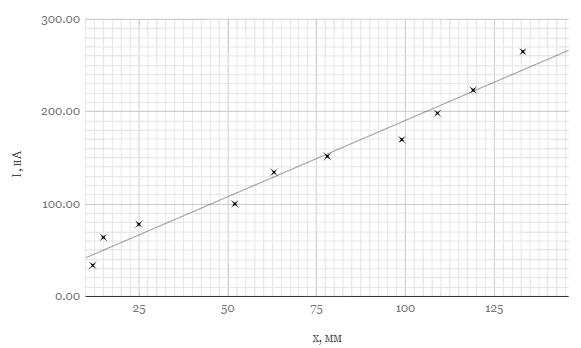
\includegraphics[width=\textwidth]{graph1.PNG}
    \caption{Определение динамической постоянной гальванометра}
    \label{fig:vac}
\end{figure}

\begin{center}
 $C_I = \frac{<xy>-<x><y>}{<x^2>-<x>^2} = 1.539$ нА/(мм/м)\\

$\sigma_{\triangle C_I} = \frac{1}{\sqrt{n}} \sqrt{\frac{<y^2>-<y>^2}{<x^2>-<x>^2} - C_I^2} = 0.069$ нА/(мм/м)  
\end{center}

Итого получаем
\begin{center}
    $C_I = 1.539 \pm 0.069$ нА/(мм/м)
\end{center}

\item Рассчитаем логарифмический декремент затухания свободных колебаний рамки разомкнутого гальванометра. Результаты измерений занесём в табл. 2. Также определим приблизительно период свободных колебаний рамки.

    \begin{table}[h]
    \centering
    \begin{center}
    \caption{Отклонения рамки при свободных колебаниях}
    \end{center}
    \vspace{0.1cm}
    \label{tab:my_label}
    \begin{tabular}{ |p{1.2cm}|p{1.2cm}|p{1.2cm}|p{1.2cm}|p{1.2cm}|p{1.2cm}|p{1.2cm}|p{1.2cm}|p{1.2cm}|p{1.2cm}|}
 \hline
    $x_1$, мм & $x_2$, мм & $x_3$, мм & $x_4$, мм & $\Theta_1$ & $\Theta_2$ & $\Theta_3$ & $\Theta$ & $\sigma_\Theta$, мм & $T$, c  \\
\hline
    14.3 & 13.4 & 12.6 & 11.8 & 0.0650 & 0.0616 & 0.0656 & 0.0641  & 0.0013 & 5\\
\hline
    \end{tabular}
\end{table} 

Получили значение логарифмического декремента затухания свободных колебаний рамки
\begin{center}
   $\Theta = 0.0641 \pm 0.0013$ 
\end{center}

\item При разомкнутом ключе $K_3$ определим наибольшее сопротивление магазина $R$, при котором при размыкании ключа зайчик не переходит за нулевое значение шкалы. Это сопротивление близко к критическому $R_c_r \approx 1000$ Ом.

\item Установим сопротивление магазина $R \approx 3R_c_r$ и подберем делитель так, чтобы в стационарном режиме зайчик отклонялся на всю шкалу. Для расчёта $\Theta$ будем измерять два последовательных отклонения зайчика в одну сторону. Повторим измерения, увеличивая сопротивление магазина до $8R_c_r$. Результаты занесём в табл. 3.

    \begin{table}[h]
    \centering
    \begin{center}
    \caption{Зависимость отклонения зайчика от сопротивления, после размыкания ключа $K_3$}
    \end{center}
    \vspace{0.1cm}
    \label{tab:my_label}
    \begin{tabular}{ |p{1.5cm}||p{1cm}|p{1cm}|p{1cm}|p{1cm}|p{1cm}|p{1cm}|p{1cm}|p{1cm}|p{1cm}| }
\hline
    $R$, кОм & 3 & 3.5 & 4 & 4.5 & 5 & 5.5 & 6 & 7 & 8  \\
\hline
    $x1$, мм & 222 & 204 & 188 & 178 & 168 & 159 & 151 & 137 & 126 \\
\hline
    $x2$, мм & 17 & 30 & 28 & 32 & 35 & 38 & 39 & 42 & 43 \\
\hline
    $\Theta$ & 2.569 & 1.917 & 1.904 & 1.716 & 1.569 & 1.431 & 1.354 & 1.182 & 1.075 \\
\hline

    \end{tabular}
\end{table}   

Построим график зависимости декремента затухания колебаний от сопротивления на магазине в координатах $1/\Theta^2 = f[(R+R_0)^2]$ (рис. 4). Используя формулу (4) и метод наименьших квадратов, определим по нему критическое сопротивление гальванометра. Также используя метода наименьших квадратов, оценим погрешность определения этой величины (формулы см. в п. 5.1)

\begin{figure}[h]
    \centering
    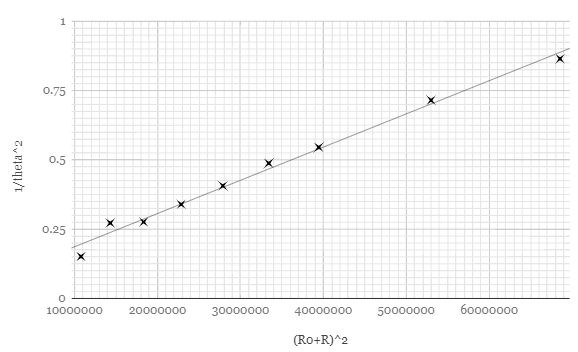
\includegraphics[width=\textwidth]{graph2.PNG}
    \caption{Определение критического сопротивления гальванометра, статический режим}
    \label{fig:vac}
\end{figure}

\begin{center}
    $R_c_r = \frac{1}{2\pi}\sqrt{\frac{\triangle X}{\triangle Y}} - R_0$ \\
    $R_c_r = 1173 \pm 25$ Ом
\end{center}

\item Перейдём к работе гальванометра в баллистическом режиме. Соберём схему по рис. 2. Разомкнём цепь $R$, отсоединив одну из клемм от магазина. Подберём делитель так, чтобы первый отбор соответствовал отклонению зайчика на всю школу. Для свободных колебаний $l_{max} = 237.8$ мм. \par
Подключим магазин назад. Снимем зависимость величины первого отброса от $R$. Результаты занесём в табл. 4.


    \begin{table}[h]
    \centering
    \begin{center}
    \caption{Зависимость отклонения зайчика от сопротивления, после размыкания ключа $K_3$}
    \end{center}
    \vspace{0.1cm}
    \label{tab:my_label}
    \begin{tabular}{ |p{1.5cm}||p{1cm}|p{1cm}|p{1cm}|p{1cm}|p{1cm}|p{1cm}|p{1cm}| }
\hline

    $l_{max}$, мм & 180 & 182 & 178 & 177 & 163 & 115 & 85 \\
\hline
    $R$, кОм & 50 & 40 & 30 & 20 & 5 & 2 & 0.8 \\
\hline

    \end{tabular}
\end{table} 

Построим график $l_{max} = f[(R_0 + R)^{-1}]$. По графику, используя метод наименьших квадратов, определим критическое сопротивление гальванометра ($l_c_r = l_{max}/e$).
\begin{figure}[h]
    \centering
    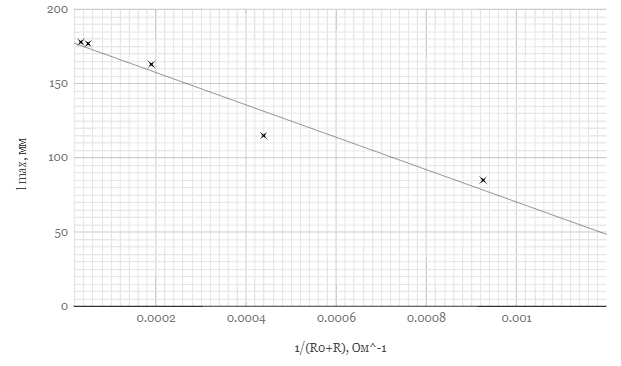
\includegraphics[width=\textwidth]{graph3.PNG}
    \caption{Определение критического сопротивления гальванометра, баллистический режим}
    \label{fig:vac}
\end{figure}

\begin{center}
    $a = 181, b = -111634$ \par
    $R_c_r = (\frac{l_c_r - a}{b})^-^1 - R_0 = 881.73 \pm 88.17$ Ом
\end{center}

\item По формуле (5) рассчитаем баллистическую постоянную в критическом режиме:
\begin{center}
    $C_Q_c_r = \frac{q}{\varphi_{max cr}} = 2a\frac{R_1}{R_2} \frac{U_0 C}{l_{max cr}}$ \par
    
    $C_Q_c_r = 9.33 \pm 0.3 * 10^-^9$ К/(мм/м)
\end{center}

\item Сравним время релаксации $t = R_0 C$ и период свободных колебаний гальванометра $T_0$
\begin{center}
    $t = 0.00056 c \ll T = 5 c$
\end{center}
Время релаксации много меньше периода свободных колебаний. Эксперимент корректен.

\end{enumerate}

\section{Вывод}

В ходе эксперимента был исследован принцип работы гальванометра в режиме постоянного тока и в баллистическом режиме. Определены динамическая и баллистическая постоянные гальванометра:

\begin{center}
    $C_I = 1.539 \pm 0.069$ нА/(мм/м) \hspace{1cm} $C_Q_c_r = 9.33 \pm 0.3 * 10^-^9$ К/(мм/м)
\end{center}

Тремя разными способами было исследовано критическое сопротивление гальванометра. Результаты практически совпадают.

    \begin{table}[h]
    \centering
    \begin{center}
    \caption{Значения $R_c_r$, полученные разными способами}
    \end{center}
    \vspace{0.1cm}
    \label{tab:my_label}
    \begin{tabular}{ |p{4cm}|p{4cm}|p{4cm}|}
 \hline
    $R_c_r$, Ом - подбор & $R_c_r$, Ом  - по графику в стационарном режиме & $R_c_r$, Ом - по графику в баллистическом режиме \\
\hline
    $1000$ & $1173 \pm 25$ & $882 \pm 88$ \\
\hline
    \end{tabular}
\end{table} 

\end{document}
